Am nähesten zu der \textbf{PAC}\footnote{Port-Adapter-Controller} Struktrur 
ist das Pattern \textbf{MVP}\footnote{Model-View-Presenter}.
Dabei die Aufgaben von \textbf{View} entsprechen den Aufgaben von \textbf{Port}. 
Die Aufgaben von \textbf{Presenter} entsprechen den Aufgaben \textbf{Adapter}.
Und die Aufgaben von dem Rest des Programms inklusiv \textbf{Controller} entspechen den Aufgaben von \textbf{Model}.

Der Unterschied zu \textbf{MVP} besteht darin, dass \textbf{MVP} im klassischen Sinne nur für die Benutzerobeflächen gedacht ist,
während in der hier beschriebenen Umsetzung wird es für alle Schnittstellen benutzt.
\textbf{MVP} Architektur übernimmt in der gesamten Application eine zentralle Stelle und ist nur einmal zu treffen.
\textbf{PAC} ist nur ein Teil der gesamten Application, wird an mehreren Stellen unterschiedlich benutzt und beschreibt nicht 
die Architektur der Application.


\begin{figure}[H]
   \centering
   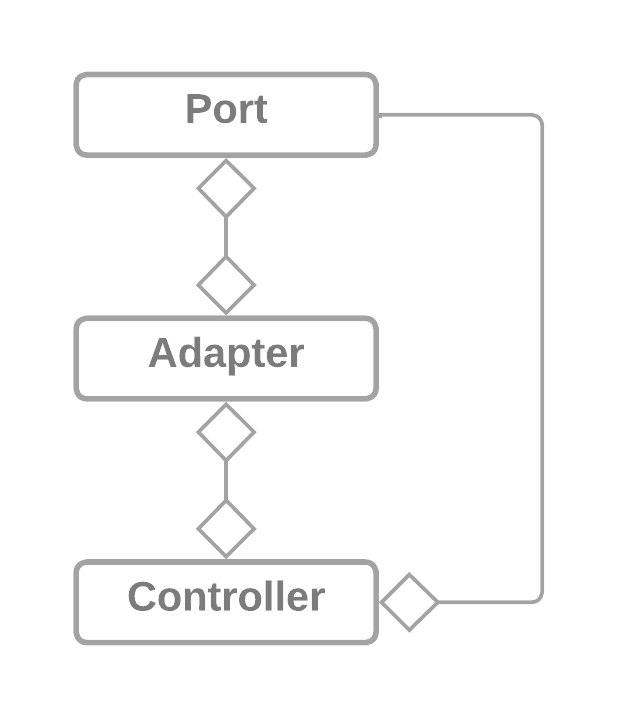
\includegraphics[width=6.5cm]{./images/Port-Adapter-Contoller.png}
    \caption[Objektendiagramm PAC]{Objektendiagramm PAC \footnotemark}
    \label{fig:CDPAC}
\end{figure}
\footnotetext{Eigene Quelle}